 \documentclass[oneside,11pt]{article}


\usepackage{soul}
\usepackage{natbib}
\usepackage{hyperref}
\usepackage{bookmark}
\usepackage{graphicx}             
\graphicspath{{./Figuras/}}
\usepackage[dvipsnames]{xcolor}
\usepackage{todonotes}
\usepackage{makecell}
\usepackage[margin=1in]{geometry}
\usepackage{float}                
\usepackage{amsmath}
\usepackage{amscd}
\usepackage{amsfonts}
\usepackage{amssymb}
\usepackage{bbm}
\usepackage{booktabs}
\usepackage{nameref}
\usepackage{multirow}
\usepackage[nokeyprefix]{refstyle}
\usepackage{rotating}
\usepackage{threeparttable}
\usepackage{afterpage}
\usepackage{lscape}
\usepackage{enumerate}
\usepackage{caption}
\usepackage{subcaption}
\usepackage{epstopdf}
\usepackage{setspace}
\usepackage{svg}
\usepackage{dsfont}
\usepackage{amsthm}
\usepackage{tocloft}
\usepackage{etoc}
\usepackage{lmodern}
\usepackage{bm}
\usepackage[T1]{fontenc}
\usepackage{tgpagella}

\epstopdfDeclareGraphicsRule{.tiff}{png}{.png}{convert #1 \OutputFile}
\AppendGraphicsExtensions{.tiff}

\epstopdfDeclareGraphicsRule{.tif}{png}{.png}{convert #1 \OutputFile}
\AppendGraphicsExtensions{.tif}

\def\sym#1{\ifmmode^{#1}\else\(^{#1}\)\fi}

\usepackage{tikz}
\usetikzlibrary{shapes.geometric, arrows}
\usetikzlibrary{calc}
\usetikzlibrary{matrix}

\tikzset{ 
    table/.style={
        matrix of nodes,
        row sep=-\pgflinewidth,
        column sep=-\pgflinewidth,
        nodes={
            rectangle,
            draw=black,
            align=center
        },
        minimum height=1.5em,
        text depth=0.5ex,
        text height=2ex,
        nodes in empty cells,
%%
        every even row/.style={
            nodes={fill=gray!20}
        },
        column 1/.style={
            nodes={text width=2em,font=\bfseries}
        },
        row 1/.style={
            nodes={
                fill=black,
                text=white,
                font=\bfseries
            }
        }
    }
}


\usepackage{colortbl}
\usepackage{url}
\urlstyle{rm}
\definecolor{darkblue}{rgb}{0,0,.4}
\hypersetup{colorlinks=true, breaklinks=true, citecolor=Maroon, linkcolor=darkblue, menucolor=darkblue, urlcolor=darkblue}

\newtheorem{theorem}{Theorem}
\newtheorem{claim}[theorem]{Claim}
\newtheorem{prop}[theorem]{Proposition} 
\newtheorem{cor}[theorem]{Corollary} 
\newtheorem{assumption}{Assumption} 
\newtheorem{lem}{Lemma} 

\DeclareRobustCommand{\hlgr}[1]{{\sethlcolor{green}\hl{#1}}}


\usepackage{comment}
%para esconder columnas en tablas (enrique)
\usepackage{array}
\newcolumntype{H}{>{\setbox0=\hbox\bgroup}c<{\egroup}@{}}
\linespread{1.25}

\newcommand{\wh}{\widehat}
\usepackage{anyfontsize}

\usepackage[linesnumbered,vlined,ruled,commentsnumbered]{algorithm2e}

\DontPrintSemicolon
\newcommand{\To}{\mbox{\upshape\bfseries to}}
\newcommand{\E}{\mathbb{E}}

\DeclareCaptionFormat{cont}{#1 (cont.)#2#3\par}
%%% HELPER CODE FOR DEALING WITH EXTERNAL REFERENCES
\usepackage{xr}
\makeatletter
\newcommand*{\addFileDependency}[1]{
  \typeout{(#1)}
  \@addtofilelist{#1}
  \IfFileExists{#1}{}{\typeout{No file #1.}}
}
\makeatother


\newcommand*{\myexternaldocument}[1]{
    \externaldocument{#1}
    \addFileDependency{#1.tex}
    \addFileDependency{#1.aux}
}

%\myexternaldocument{OA}

%%%%%%%%%%%%%%%%%%%%%%%%%%%%%%%% DOCUMENT
\begin{document}

\title{IMSS RPCI \thanks{We want to thank.}}
\author{Eduardo Alcaraz \and Gabriela López \and Luis Martínez \and Marco Medina \and Enrique Seira  \thanks{Seira: ITAM, enrique.seira@gmail.com (corresponding author); Alcaraz: IMSS, eduardo.alcarazp@imss.gob.mx; López: IMSS, ; Martínez: IMSS, luis.martinezch@imss.gob.mx; Medina:  ITAM, marco.medina@itam.mx}}
\date{This draft:  \today \\[2 cm]}

%\vspace{.5in}


\maketitle
\thispagestyle{empty}
\begin{abstract}

%Abstract here. 

\end{abstract}

\vspace{.3in}

\textbf{Keywords: }

\textbf{JEL codes:}

\newpage

\pagenumbering{arabic}
\etocdepthtag.toc{mtchapter}
\etocsettagdepth{mtchapter}{subsection}
\etocsettagdepth{mtappendix}{none}





%\FloatBarrier
%%%%%%%%%%%%%%%%%%%%%%%%%%%%%%%%%%%%%%%%

\clearpage
\singlespacing

\section{Tables}

\begin{table}[H]
    \caption{Balance table}
    \label{balance_1}
    \begin{center}
    \scriptsize{% Table generated by Excel2LaTeX from sheet 'SelfUpdate_balance_1'
\begin{tabular}{r|rrr}
\toprule
\toprule
\multicolumn{1}{p{12.085em}|}{} & \multicolumn{1}{c}{Worker didn't} & \multicolumn{1}{c}{Worker} &  \\
\multicolumn{1}{p{12.085em}|}{Variables} & \multicolumn{1}{c}{Downloaded RPCI} & \multicolumn{1}{c}{Downloaded RPCI} & \multicolumn{1}{c}{t-test} \\
\midrule
\multicolumn{1}{p{12.085em}|}{} &                 &                 &  \\
\multicolumn{1}{p{12.085em}|}{Women} & \multicolumn{1}{c}{0.394} & \multicolumn{1}{c}{0.404} & \multicolumn{1}{c}{0.010*} \\
\multicolumn{1}{p{12.085em}|}{} & \multicolumn{1}{c}{(0.489)} & \multicolumn{1}{c}{(0.491)} & \multicolumn{1}{c}{(0.005)} \\
\multicolumn{1}{p{12.085em}|}{Wage} & \multicolumn{1}{c}{365.076} & \multicolumn{1}{c}{387.122} & \multicolumn{1}{c}{22.046***} \\
                & \multicolumn{1}{c}{(375.164)} & \multicolumn{1}{c}{(379.881)} & \multicolumn{1}{c}{(4.496)} \\
\multicolumn{1}{p{12.085em}|}{Temporary worker} & \multicolumn{1}{c}{0.169} & \multicolumn{1}{c}{0.150} & \multicolumn{1}{c}{-0.019***} \\
\multicolumn{1}{p{12.085em}|}{} & \multicolumn{1}{c}{(0.375)} & \multicolumn{1}{c}{(0.357)} & \multicolumn{1}{c}{(0.004)} \\
\multicolumn{1}{p{12.085em}|}{Government} & \multicolumn{1}{c}{0.066} & \multicolumn{1}{c}{0.079} & \multicolumn{1}{c}{0.013***} \\
\multicolumn{1}{p{12.085em}|}{} & \multicolumn{1}{c}{(0.249)} & \multicolumn{1}{c}{(0.270)} & \multicolumn{1}{c}{(0.003)} \\
\multicolumn{1}{p{12.085em}|}{Outsourcing} & \multicolumn{1}{c}{0.251} & \multicolumn{1}{c}{0.292} & \multicolumn{1}{c}{0.041***} \\
                & \multicolumn{1}{c}{(0.434)} & \multicolumn{1}{c}{(0.455)} & \multicolumn{1}{c}{(0.005)} \\
\multicolumn{1}{p{12.085em}|}{Agriculture} & \multicolumn{1}{c}{0.048} & \multicolumn{1}{c}{0.013} & \multicolumn{1}{c}{-0.036***} \\
\multicolumn{1}{p{12.085em}|}{} & \multicolumn{1}{c}{(0.214)} & \multicolumn{1}{c}{(0.111)} & \multicolumn{1}{c}{(0.003)} \\
\multicolumn{1}{p{12.085em}|}{Extractive Ind.} & \multicolumn{1}{c}{0.006} & \multicolumn{1}{c}{0.006} & \multicolumn{1}{c}{-0.000} \\
\multicolumn{1}{p{12.085em}|}{} & \multicolumn{1}{c}{(0.077)} & \multicolumn{1}{c}{(0.076)} & \multicolumn{1}{c}{(0.001)} \\
\multicolumn{1}{p{12.085em}|}{Transformation Ind.} & \multicolumn{1}{c}{0.261} & \multicolumn{1}{c}{0.204} & \multicolumn{1}{c}{-0.057***} \\
\multicolumn{1}{p{12.085em}|}{} & \multicolumn{1}{c}{(0.439)} & \multicolumn{1}{c}{(0.403)} & \multicolumn{1}{c}{(0.005)} \\
\multicolumn{1}{p{12.085em}|}{Construction Ind.} & \multicolumn{1}{c}{0.099} & \multicolumn{1}{c}{0.081} & \multicolumn{1}{c}{-0.018***} \\
\multicolumn{1}{p{12.085em}|}{} & \multicolumn{1}{c}{(0.299)} & \multicolumn{1}{c}{(0.273)} & \multicolumn{1}{c}{(0.004)} \\
\multicolumn{1}{p{12.085em}|}{Electric Ind.} & \multicolumn{1}{c}{0.006} & \multicolumn{1}{c}{0.007} & \multicolumn{1}{c}{0.000} \\
\multicolumn{1}{p{12.085em}|}{} & \multicolumn{1}{c}{(0.078)} & \multicolumn{1}{c}{(0.081)} & \multicolumn{1}{c}{(0.001)} \\
\multicolumn{1}{p{12.085em}|}{Commerce} & \multicolumn{1}{c}{0.196} & \multicolumn{1}{c}{0.227} & \multicolumn{1}{c}{0.031***} \\
                & \multicolumn{1}{c}{(0.397)} & \multicolumn{1}{c}{(0.419)} & \multicolumn{1}{c}{(0.005)} \\
\multicolumn{1}{p{12.085em}|}{Transport} & \multicolumn{1}{c}{0.056} & \multicolumn{1}{c}{0.062} & \multicolumn{1}{c}{0.006**} \\
\multicolumn{1}{p{12.085em}|}{} & \multicolumn{1}{c}{(0.229)} & \multicolumn{1}{c}{(0.240)} & \multicolumn{1}{c}{(0.003)} \\
\multicolumn{1}{p{12.085em}|}{Personal services} & \multicolumn{1}{c}{0.232} & \multicolumn{1}{c}{0.293} & \multicolumn{1}{c}{0.061***} \\
\multicolumn{1}{p{12.085em}|}{} & \multicolumn{1}{c}{(0.422)} & \multicolumn{1}{c}{(0.455)} & \multicolumn{1}{c}{(0.005)} \\
\multicolumn{1}{p{12.085em}|}{Social services} & \multicolumn{1}{c}{0.095} & \multicolumn{1}{c}{0.109} & \multicolumn{1}{c}{0.013***} \\
\multicolumn{1}{p{12.085em}|}{} & \multicolumn{1}{c}{(0.294)} & \multicolumn{1}{c}{(0.311)} & \multicolumn{1}{c}{(0.004)} \\
\midrule
\multicolumn{1}{p{12.085em}|}{Observations} & \multicolumn{1}{c}{316,807} & \multicolumn{1}{c}{8,585} & \multicolumn{1}{c}{325,392} \\
                &                 &                 &  \\
\bottomrule
\bottomrule
\end{tabular}%
}
    %\textit{Do file: balance_rpci.do}
    \end{center}
\end{table}

\scriptsize{
\noindent Random sample of the workers registered at the Mexican Institute of Social Security (IMSS) between January 2020 and August 2022. Balance table elaborated with the workers' characteristics during 2020, before the launch of the RPCI app.
}

\clearpage

\subsection{TWFE}

\begin{table}[H]
    \caption{RPCI effect on wage}
    \label{twfe_wage}
    \begin{center}
    \scriptsize{% Table generated by Excel2LaTeX from sheet 'twfe_wage'
\begin{tabular}{ccccccc}
\toprule
\toprule
      & (1)   & (2)   & (3)   & (4)   & (5)   & (6) \\
\cmidrule{2-7}      & \multicolumn{6}{c}{\textit{A) Wage}} \\
\midrule
RPCI  & 9.3*** & 6.3*** & 8.6*** & 8.2*** & 9.3*** & 4.9*** \\
      & (0.68) & (0.71) & (0.71) & (0.71) & (0.71) & (0.70) \\
Constant & 435.8*** & 447.6*** & 447.6*** & 447.6*** & 447.6*** & 447.6*** \\
      & (0.01) & (0.01) & (0.01) & (0.01) & (0.01) & (0.01) \\
Mean  & 435.9 & 447.7 & 447.7 & 447.7 & 447.7 & 447.7 \\
\cmidrule{2-7}      & \multicolumn{6}{c}{\textit{B) Log Wage}} \\
\midrule
RPCI  & 0.02*** & 0.01*** & 0.02*** & 0.02*** & 0.02*** & 0.01*** \\
      & (0.001) & (0.001) & (0.001) & (0.001) & (0.001) & (0.001) \\
Constant & 5.77*** & 5.80*** & 5.80*** & 5.80*** & 5.80*** & 5.80*** \\
      & (0.000) & (0.000) & (0.000) & (0.000) & (0.000) & (0.000) \\
Mean  & 5.77  & 5.80  & 5.80  & 5.80  & 5.80  & 5.80 \\
\midrule
Observations & 63,753,101 & 59,094,387 & 59,094,387 & 59,094,387 & 59,085,813 & 59,085,813 \\
Workers & 3,066,419 & 2,487,384 & 2,487,384 & 2,487,384 & 2,486,270 & 2,486,270 \\
Firms & 597,071 & 539,898 & 539,898 & 539,898 & 539,737 & 539,737 \\
\midrule
\textit{Linear Trends FE} &       &       &       &       &       &  \\
Age   &       & \checkmark &       &       &       & \checkmark \\
Firm Industry &       &       & \checkmark &       &       & \checkmark \\
State &       &       &       & \checkmark &       & \checkmark \\
Wage Decile &       &       &       &       & \checkmark & \checkmark \\
\bottomrule
\bottomrule
\end{tabular}%
}
    %\textit{Do file: twfe_rpci.do}
    \end{center}
\end{table}

\scriptsize{
\noindent This table shows the effect of registering to the RPCI on the reported wage. \textit{Sample:} 10\%of the workers registered at the Mexican Institute of Social Security (IMSS) between January 2020 and August 2022. Regressions use the TWFE specification $y_{it} = \gamma_{i} + \theta_{t}+ \beta RPCI_{it} +\epsilon_{it}$, where $\gamma_{i}$ are dummies for each worker id, $\theta_{t}$ are dummies for each monthly period, and $RPCI_{it}$ are dummies where 1 means that the worker registered for the RPCI during that month or previous month. Regressions on columns (2)-(6) include fixed effects on linear trends, by interacting dummies on worker's baseline characteristics with a set of dummies for each quarterly period: (2) age group, (3) firm industry, (4) state, (5) wage decile, (6) all previous. Robust standard errors clustered by worker id in parenthesis. *** $p<0.01$, ** $p<0.05$, * $p<0.1$.
}


\clearpage


\begin{table}[H]
    \caption{RPCI effect on being enrolled, enrollments, discharges, wage and job changes}
    \label{twfe_job}
    \begin{center}
    \scriptsize{% Table generated by Excel2LaTeX from sheet 'twfe_job'
\begin{tabular}{c|cHHHcc}
\toprule
\toprule
      & Enrolled & Enrollment & Discharge & Perm. Discharge & Wage Change & Job Change \\
Variables & (1) & (2) & (3) & (4) & (2) & (3) \\
\midrule
      &       &       &       &       &       &  \\
RPCI  & 0.046*** & 0.001*** & 0.011*** & 0.010*** & 0.003*** & 0.004*** \\
      & (0.001) & (0.000) & (0.000) & (0.000) & (0.001) & (0.000) \\
Constant & 0.725*** & 0.025*** & 0.029*** & 0.010*** & 0.327*** & 0.025*** \\
      & (0.000) & (0.000) & (0.000) & (0.000) & (0.000) & (0.000) \\
      &       &       &       &       &       &  \\
\midrule
Observations & 81,552,640 & 81,552,640 & 81,552,640 & 81,552,640 & 56,408,801 & 56,408,801 \\
Mean  & 0.726 & 0.025 & 0.029 & 0.010 & 0.327 & 0.025 \\
Workers & 2,548,520 & 2,548,520 & 2,548,520 & 2,548,520 & 2,423,821 & 2,423,821 \\
Firms & 544,282 & 544,282 & 544,282 & 544,282 & 520,132 & 520,132 \\
\bottomrule
\bottomrule
\end{tabular}%
}
    %\textit{Do file: twfe_rpci.do}
    \end{center}
\end{table}

\scriptsize{
\noindent \textit{Sample:} 10\%of the workers registered at the Mexican Institute of Social Security (IMSS) between January 2020 and August 2022. \textit{Enrolled} is a dummy where 1 means the worker had a job registered during period $t$. \textit{Enrollment} is a dummy where 1 means the worker had a job registered during period $t$, but didn't have one during period $t-1$. \textit{Discharge} is a dummy where 1 means the worker had a job registered during period $t$, but didn't have one during period $t+1$. \textit{Permanent Discharge} is a dummy where 1 means the worker had a register during period $t$, but never had a job registered again for the rest of the months in the sample. \textit{Wage Change} is a dummy where 1 means the worker had a job registered during period $t$, and had a job registered with a different wage during period $t+1$. \textit{Job Change} is a dummy where 1 means the worker had a job registered during period $t$, and had a job registered at a different firm during period $t+1$. Regressions use the TWFE specification $y_{it} = \gamma_{i} + \theta_{t}+ \beta RPCI_{it} +\epsilon_{it}$, where $\gamma_{i}$ are dummies for each worker id, $\theta_{t}$ are dummies for each monthly period, and $RPCI_{it}$ are dummies where 1 means that the worker registered for the RPCI during that month or previous month. Regressions include fixed effects on linear trends for age group, firm industry, state and wage decile, by interacting dummies on worker's baseline characteristics with a set of dummies for each quarterly period. Robust standard errors clustered by worker id in parenthesis. *** $p<0.01$, ** $p<0.05$, * $p<0.1$.
}

\clearpage



\subsection{TWFE - Heterogeneity}

\begin{table}[H]
    \caption{RPCI effect on wage by worker characteristics}
    \label{twfe_wage_hetero_wrk_char}
    \begin{center}
    \scriptsize{% Table generated by Excel2LaTeX from sheet 'twfe_wage_hetero_wrk_char'
\begin{tabular}{ccccc}
\toprule
\toprule
      & Men   & Women & Outsourcing & Temporary \\
      & (1)   & (2)   & (3)   & (4) \\
\cmidrule{2-5}      & \multicolumn{4}{c}{\textit{B) Log Wage}} \\
\midrule
RPCI  & 0.02*** & 0.01*** & 0.00  & 0.01*** \\
      & (0.002) & (0.002) & (0.002) & (0.003) \\
Constant & 5.83*** & 5.74*** & 5.96*** & 5.74*** \\
      & (0.000) & (0.000) & (0.000) & (0.000) \\
Mean  & 5.83  & 5.74  & 5.96  & 5.74 \\
\midrule
Observations & 36,408,980 & 22,676,833 & 15,323,763 & 8,282,504 \\
Workers & 1,536,994 & 949,276 & 633,118 & 411,987 \\
Firms & 421,422 & 283,428 & 125,402 & 145,157 \\
\bottomrule
\bottomrule
\end{tabular}%
}
    %\textit{Do file: twfe_rpci_heterogeneity.do}
    \end{center}
\end{table}
\scriptsize{
\noindent This table looks into heterogeneity in the RPCI effect by worker characteristics. Each column conditions on a worker characteristics at baseline, during 2020, previous to the RPCI launch. Columns (1) and (2) condition on the worker gender. Column (3) conditions on workers hired through outsourcing. Column (4) conditions on temporary workers. \textit{Sample:} 10\%of the workers registered at the Mexican Institute of Social Security (IMSS) between January 2020 and August 2022. Regressions use the TWFE specification $y_{it} = \gamma_{i} + \theta_{t}+ \beta RPCI_{it} +\epsilon_{it}$, where $\gamma_{i}$ are dummies for each worker id, $\theta_{t}$ are dummies for each monthly period, and $RPCI_{it}$ are dummies where 1 means that the worker registered for the RPCI during that month or previous month. Regressions include fixed effects on linear trends for age group, firm industry, state and wage decile, by interacting dummies on worker's baseline characteristics with a set of dummies for each quarterly period. Robust standard errors clustered by worker id in parenthesis. *** $p<0.01$, ** $p<0.05$, * $p<0.1$.
}

\clearpage


\begin{landscape}

\begin{table}[H]
    \caption{RPCI effect on wage by firm characteristics}
    \label{twfe_wage_hetero_firm_char}
    \begin{center}
    \scriptsize{% Table generated by Excel2LaTeX from sheet 'twfe_wage_hetero_firm_char'
\begin{tabular}{c|cccccccc}
\toprule
\toprule
      & \multicolumn{8}{c}{Wage} \\
\midrule
      & (1)   & (2)   & (3)   & (4)   & (5)   & (6)   & (7)   & (8) \\
      & Transf. Ind. & Constr. Ind. & Commerce & Transport & Pers. Serv. & Soc. Serv. & Small Firm & Big Firm \\
\midrule
      &       &       &       &       &       &       &       &  \\
RPCI  & 4.695*** & 20.930*** & 5.805*** & 9.393*** & 7.252*** & 7.742*** & 3.146*** & 8.782*** \\
      & (1.208) & (2.216) & (1.262) & (2.610) & (1.393) & (1.516) & (0.791) & (1.266) \\
Constant & 463.650*** & 317.290*** & 387.124*** & 478.685*** & 456.057*** & 575.509*** & 360.735*** & 567.809*** \\
      & (0.079) & (0.166) & (0.101) & (0.205) & (0.120) & (0.124) & (0.056) & (0.097) \\
      &       &       &       &       &       &       &       &  \\
\midrule
Observations & 1,638,609 & 443,306 & 1,200,840 & 353,243 & 1,342,456 & 663,941 & 3,000,418 & 1,567,032 \\
R-squared & 0.945 & 0.885 & 0.921 & 0.932 & 0.932 & 0.951 & 0.941 & 0.939 \\
Mean  & 463.690 & 317.530 & 387.197 & 478.799 & 456.166 & 575.619 & 360.771 & 567.914 \\
Workers & 65,310 & 24,004 & 49,399 & 14,145 & 58,126 & 24,308 & 158,757 & 62,051 \\
Firms & 35,782 & 31,312 & 39,399 & 13,752 & 50,957 & 10,113 & 137,674 & 18,857 \\
\midrule
\midrule
\multicolumn{1}{r}{} &       &       &       &       &       &       &       &  \\
\midrule
\midrule
      & \multicolumn{8}{c}{Log Wage} \\
\midrule
      & (1)   & (2)   & (3)   & (4)   & (5)   & (6)   & (7)   & (8) \\
      & Transf. Ind. & Constr. Ind. & Commerce & Transport & Pers. Serv. & Soc. Serv. & Small Firm & Big Firm \\
\midrule
      &       &       &       &       &       &       &       &  \\
RPCI  & 0.013*** & 0.042*** & 0.015*** & 0.025*** & 0.028*** & 0.013*** & 0.015*** & 0.018*** \\
      & (0.002) & (0.005) & (0.002) & (0.005) & (0.002) & (0.002) & (0.001) & (0.002) \\
Constant & 5.879*** & 5.514*** & 5.688*** & 5.861*** & 5.728*** & 6.096*** & 5.590*** & 6.075*** \\
      & (0.000) & (0.000) & (0.000) & (0.000) & (0.000) & (0.000) & (0.000) & (0.000) \\
      &       &       &       &       &       &       &       &  \\
\midrule
Observations & 1,638,609 & 443,306 & 1,200,840 & 353,243 & 1,342,456 & 663,941 & 3,000,418 & 1,567,032 \\
R-squared & 0.936 & 0.868 & 0.914 & 0.922 & 0.93  & 0.958 & 0.938 & 0.931 \\
Mean  & 5.879 & 5.514 & 5.689 & 5.862 & 5.729 & 6.097 & 5.591 & 6.076 \\
Workers & 65,310 & 24,004 & 49,399 & 14,145 & 58,126 & 24,308 & 158,757 & 62,051 \\
Firms & 35,782 & 31,312 & 39,399 & 13,752 & 50,957 & 10,113 & 137,674 & 18,857 \\
\bottomrule
\bottomrule
\end{tabular}%
}
    %\textit{Do file: twfe_rpci_heterogeneity.do}
    \end{center}
\end{table}
\scriptsize{
\noindent This table looks into heterogeneity in the RPCI effect by firm characteristics. Each column conditions on firm characteristics at baseline, during 2020, previous to the RPCI launch. Columns (1) to (6) condition on the firm industry: (1) transformation industry, (2) construction industry, (3) commerce, (4) communications and transportation, (5) services for firms and people, (6) communal and social services. Columns (7) and (8) condition on firm size categories: (7) small firms (less than 250 workers), (8) big firms (more than 1000 workers). \textit{Sample:} 10\%of the workers registered at the Mexican Institute of Social Security (IMSS) between January 2020 and August 2022. Regressions use the TWFE specification $y_{it} = \gamma_{i} + \theta_{t}+ \beta RPCI_{it} +\epsilon_{it}$, where $\gamma_{i}$ are dummies for each worker id, $\theta_{t}$ are dummies for each monthly period, and $RPCI_{it}$ are dummies where 1 means that the worker registered for the RPCI during that month or previous month. Regressions include fixed effects on linear trends for age group, firm industry, state and wage decile, by interacting dummies on worker's baseline characteristics with a set of dummies for each quarterly period. Robust standard errors clustered by worker id in parenthesis. *** $p<0.01$, ** $p<0.05$, * $p<0.1$.
}

\end{landscape}


\clearpage

\begin{landscape}

\begin{table}[H]
    \caption{RPCI effect on wage by firm size}
    \label{twfe_wage_hetero_firm_size}
    \begin{center}
    \scriptsize{% Table generated by Excel2LaTeX from sheet 'twfe_wage_hetero_firm_size'
\begin{tabular}{c|ccccccc}
\toprule
\toprule
      & \multicolumn{7}{c}{Wage} \\
\midrule
      & (1)   & (2)   & (3)   & (4)   & (5)   & (6)   & (7) \\
      & 1     & 2 to 5 & 6 to 50 & 51 to 250 & 251 to 500 & 501 to 1000 & 1000+ \\
\midrule
      &       &       &       &       &       &       &  \\
RPCI  & 9.257** & 16.279*** & 7.714*** & 8.159*** & 12.270*** & -6.160*** & 8.782*** \\
      & (4.152) & (1.944) & (1.171) & (1.344) & (1.880) & (2.003) & (1.266) \\
Constant & 221.209*** & 234.349*** & 327.235*** & 436.753*** & 494.817*** & 502.972*** & 567.809*** \\
      & (0.241) & (0.131) & (0.088) & (0.104) & (0.152) & (0.154) & (0.097) \\
      &       &       &       &       &       &       &  \\
\midrule
Observations & 75,014 & 327,313 & 1,229,866 & 1,379,158 & 685,335 & 647,223 & 1,567,032 \\
R-squared & 0.932 & 0.903 & 0.926 & 0.927 & 0.934 & 0.932 & 0.939 \\
Mean  & 221.271 & 234.503 & 327.322 & 436.852 & 494.973 & 502.897 & 567.914 \\
Workers & 3,213 & 14,492 & 54,226 & 59,131 & 28,758 & 26,817 & 62,051 \\
Firms & 4,155 & 20,520 & 72,900 & 53,362 & 21,618 & 15,879 & 18,857 \\
\midrule
\midrule
\multicolumn{1}{r}{} &       &       &       &       &       &       &  \\
\midrule
\midrule
      & \multicolumn{7}{c}{Log Wage} \\
\midrule
      & (1)   & (2)   & (3)   & (4)   & (5)   & (6)   & (7) \\
      & 1     & 2 to 5 & 6 to 50 & 51 to 250 & 251 to 500 & 501 to 1000 & 1000+ \\
\midrule
      &       &       &       &       &       &       &  \\
RPCI  & 0.036*** & 0.037*** & 0.024*** & 0.026*** & 0.028*** & -0.011*** & 0.018*** \\
      & (0.008) & (0.004) & (0.002) & (0.002) & (0.003) & (0.003) & (0.002) \\
Constant & 5.220*** & 5.278*** & 5.520*** & 5.773*** & 5.896*** & 5.933*** & 6.075*** \\
      & (0.000) & (0.000) & (0.000) & (0.000) & (0.000) & (0.000) & (0.000) \\
      &       &       &       &       &       &       &  \\
\midrule
Observations & 75,014 & 327,313 & 1,229,866 & 1,379,158 & 685,335 & 647,223 & 1,567,032 \\
R-squared & 0.926 & 0.911 & 0.92  & 0.919 & 0.922 & 0.922 & 0.931 \\
Mean  & 5.220 & 5.278 & 5.521 & 5.773 & 5.896 & 5.933 & 6.076 \\
Workers & 3,213 & 14,492 & 54,226 & 59,131 & 28,758 & 26,817 & 62,051 \\
Firms & 4,155 & 20,520 & 72,900 & 53,362 & 21,618 & 15,879 & 18,857 \\
\bottomrule
\bottomrule
\end{tabular}%
}
    %\textit{Do file: twfe_rpci_heterogeneity.do}
    \end{center}
\end{table}
\scriptsize{
\noindent This table looks into heterogeneity in the RPCI effect by firm size. Each column conditions on firm size at baseline, during 2020, previous to the RPCI launch: (1) 1 job, (2) 2 to 5 jobs, (3) 6 to 50 jobs, (4) 51 to 250 jobs, (5) 251 to 500 jobs, (6) 501 to 1000 jobs, (7) more than 1000 jobs. \textit{Sample:} 10\%of the workers registered at the Mexican Institute of Social Security (IMSS) between January 2020 and August 2022. Regressions use the TWFE specification $y_{it} = \gamma_{i} + \theta_{t}+ \beta RPCI_{it} +\epsilon_{it}$, where $\gamma_{i}$ are dummies for each worker id, $\theta_{t}$ are dummies for each monthly period, and $RPCI_{it}$ are dummies where 1 means that the worker registered for the RPCI during that month or previous month. Regressions include fixed effects on linear trends for age group, firm industry, state and wage decile, by interacting dummies on worker's baseline characteristics with a set of dummies for each quarterly period. Robust standard errors clustered by worker id in parenthesis. *** $p<0.01$, ** $p<0.05$, * $p<0.1$.
}

\end{landscape}

\clearpage


\singlespacing

\section{Figures}

% \begin{figure}[H]
%     \caption{Balance - Diferencias en descarga del RPCI por estado.}
%     \label{balance_ent_final}
%     \begin{center}
%     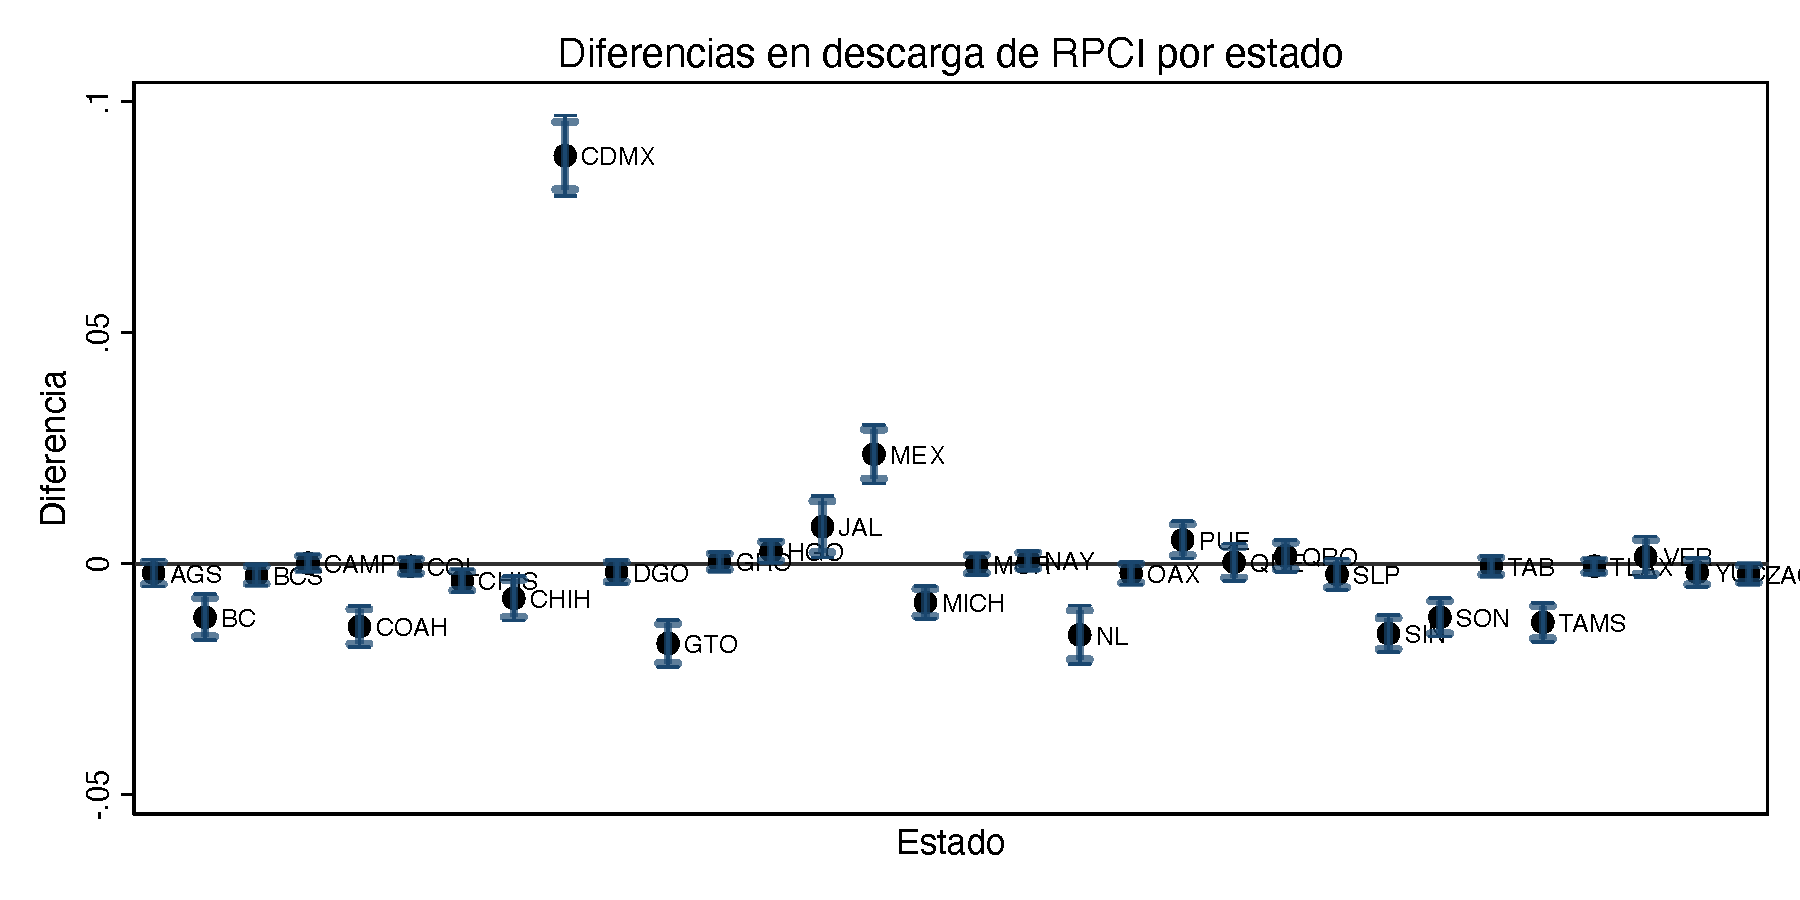
\includegraphics[width=\textwidth]{04_Figures/muestra_10porciento/balance_ent_final_graph.pdf}
%     \end{center}
% \end{figure}
% \scriptsize{
% \noindent Dado un estado, cada punto es el coeficiente resultante de correr la regresión $ent_{i} = T_{i} + \varepsilon$, donde $ent_{i}$ vale 1 si el trabajador laboraba en dicho estado en 2020, y $T_{i}$ vale 1 si el trabajador bajó el RPCI en algún momento. Es decir, dado un estado, cada punto en la figura representa la diferencia entre el porcentaje de trabajadores que bajaron el RPCI y laboran en dicho estado, y el porcentaje de trabajadores que no bajaron el RPCI y laboran en dicho estado. Por ejemplo, 25.2\% de los trabajadores que bajaron el RPCI son de CDMX, mientras que 16.4\% de los trabajadores que no bajaron el RPCI son de CDMX, por lo que la diferencia es de 8.8 pp.
% }


\vspace{.7in}
\begin{figure}[H]
    \centering
    \caption{Knowledge about IMSS and worker's reported wages \label{fig:hist_knowledge_register_survey}}
    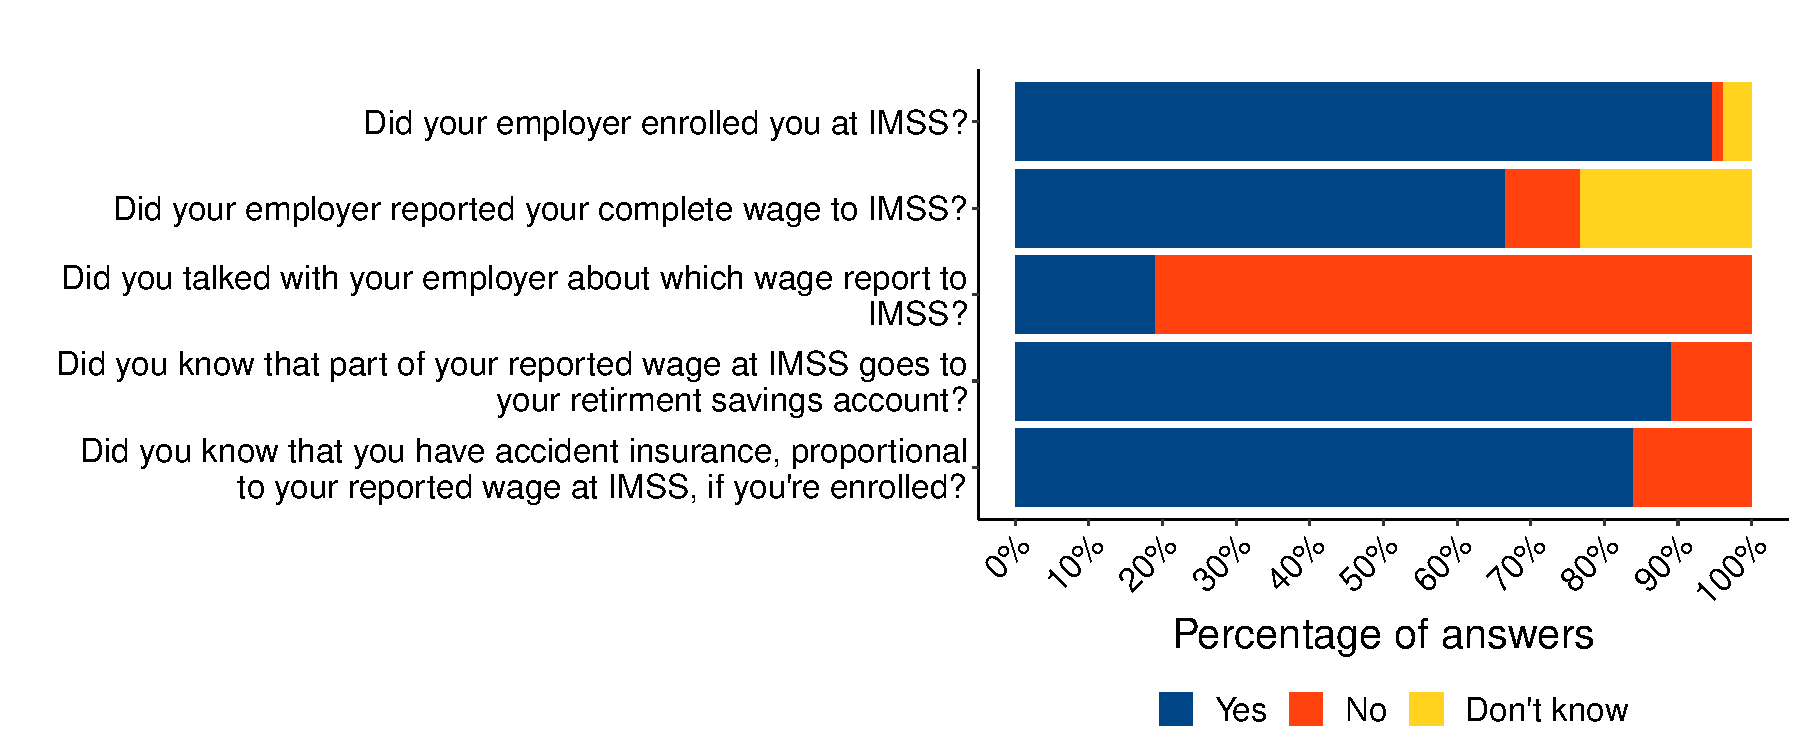
\includegraphics[width=\textwidth]{04_Figures/worker_survey/hist_knowledge_register_survey.pdf}
\end{figure}
\scriptsize{\textit{Notes}: This figure shows answers to questions about IMSS and wage reporting from the worker survey. \textit{Sample:} 233,709 answers from a survey conducted via email to workers enrolled at IMSS during August 2021. Questions 1-2, about the worker's employer, included the option "I don't know". Questions 3-5 ask about the worker's actions or knowledge didn't include the option "I don't know".}


\clearpage

\begin{figure}[H]
    \caption{RPCI registers by month}
    \label{hist_download}
    \begin{center}
    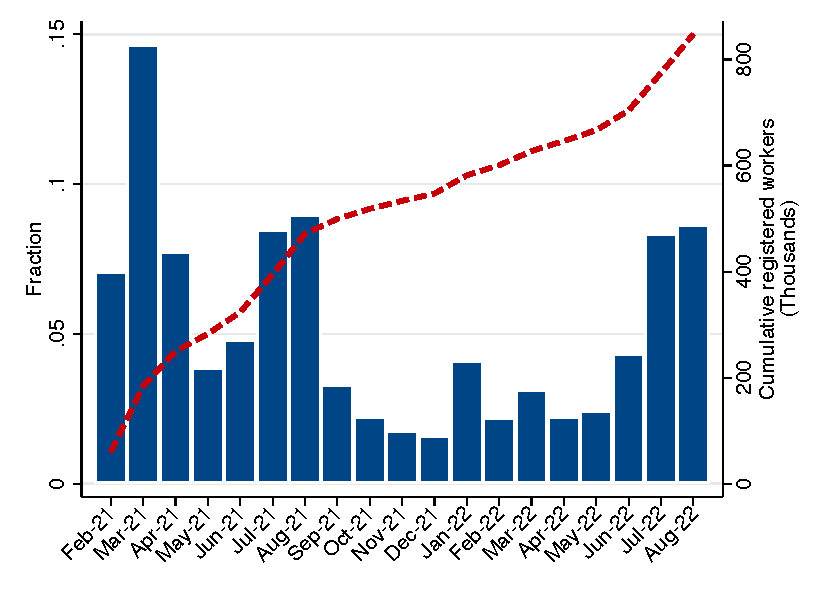
\includegraphics[width=0.75\textwidth]{04_Figures/muestra_1porciento/hist_download_month.pdf}
    \end{center}
\end{figure}
\scriptsize{
\noindent \textit{Sample:} 10\% of the workers registered at the Mexican Institute of Social Security (IMSS) between January 2020 and August 2022. The right y-axis measures the fraction of workers who registered for the RPCI during each month from the total workers who registered for the RPCI in the sample. The left y-axis measures the cumulative number of workers who registered for the RPCI in the sample.
}

\clearpage

\clearpage

\begin{figure}[H]
    \caption{Workers by the number of months observed after registering for the RPCI}
    \label{hist_time_since_treated}
    \begin{center}
    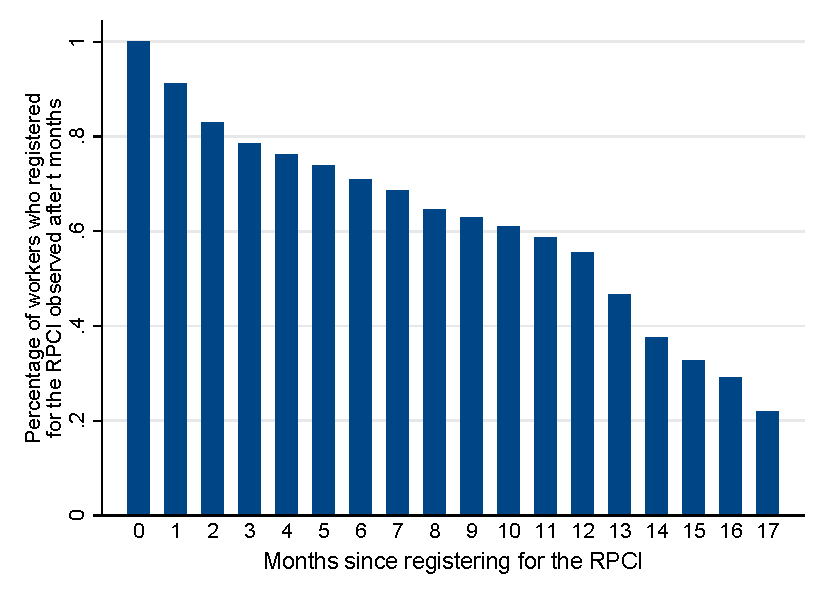
\includegraphics[width=0.7\textwidth]{04_Figures/muestra_10porciento/hist_time_since_treated.pdf}
    \end{center}
\end{figure}
\scriptsize{
\noindent \textit{Sample:} 10\% of the workers registered at the Mexican Institute of Social Security (IMSS) between January 2020 and August 2022. Not all workers registered for the RPCI at the same time, so not all workers are observed the same number of months after registering for the RPCI in the sample. The y-axis measures the percentage of workers observed $t$ months after registering for the RPCI from the total number of workers who registered for the RPCI.
}

\clearpage

\begin{figure}[H]
    \caption{Event studies - RPCI effect}
    \label{event_study}
    \begin{center}
    
    \begin{subfigure}{0.49\textwidth}
    \caption{Effect on wage}
    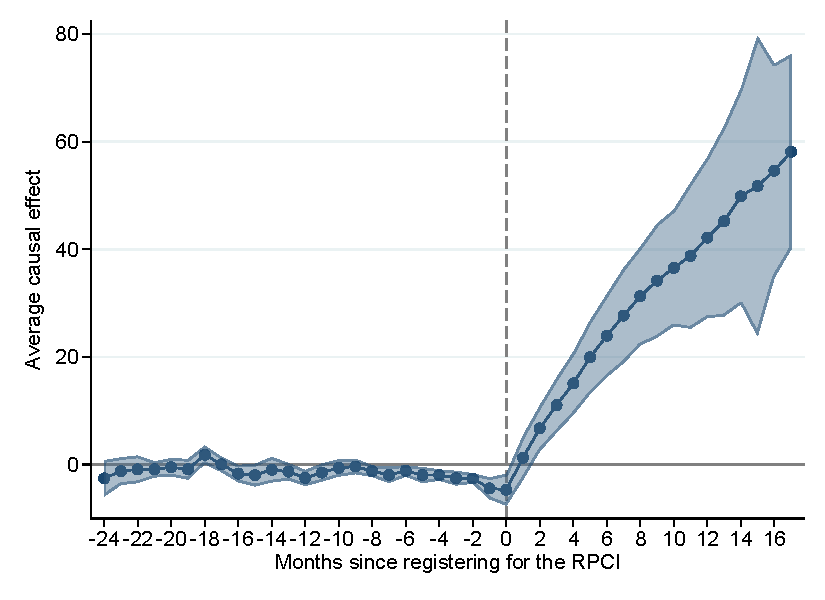
\includegraphics[width=\textwidth]{04_Figures/muestra_10porciento/event_study_sal_cierre_chaisemartin.pdf}
    \end{subfigure}
    \begin{subfigure}{0.49\textwidth}
    \caption{Effect on being enrolled}
    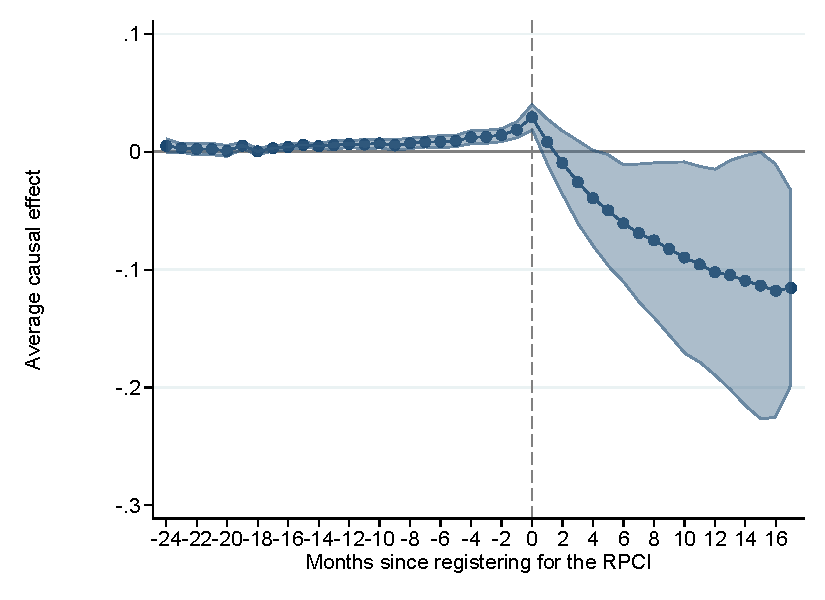
\includegraphics[width=\textwidth]{04_Figures/muestra_10porciento/event_study_alta_chaisemartin.pdf}
    \end{subfigure}
 \begin{subfigure}{0.49\textwidth}
    \caption{Effect on wage change}
    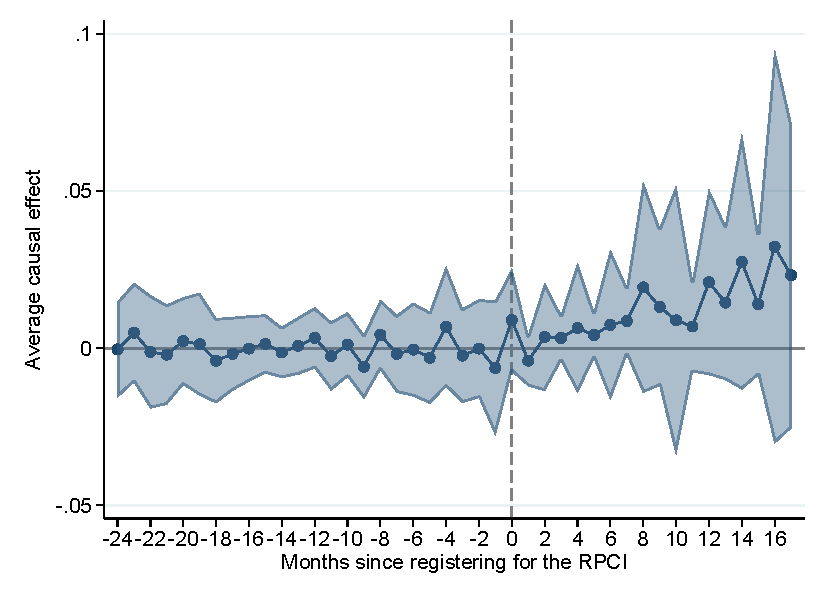
\includegraphics[width=\textwidth]{04_Figures/muestra_10porciento/event_study_sal_diff_chaisemartin.pdf}
    \end{subfigure}
    \begin{subfigure}{0.49\textwidth}
    \caption{Effect on job change}
    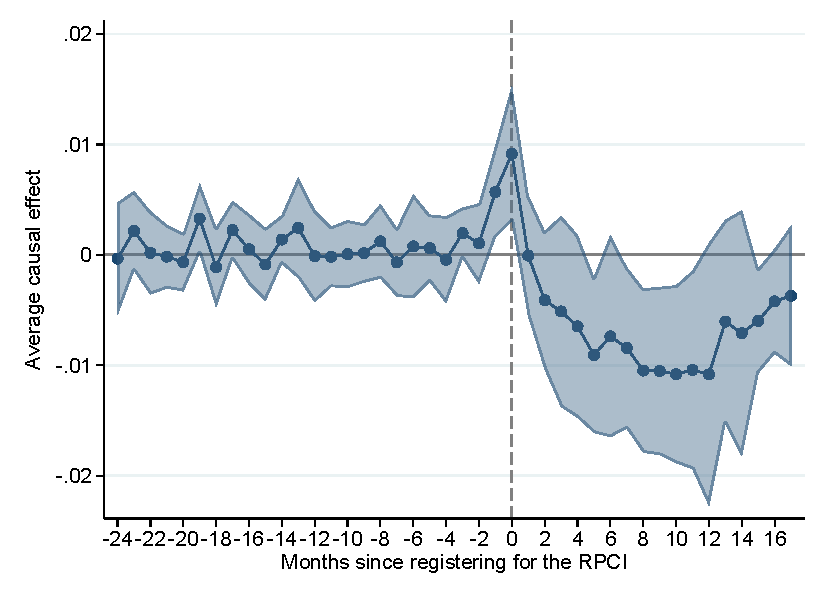
\includegraphics[width=\textwidth]{04_Figures/muestra_10porciento/event_study_cambio_cierre_chaisemartin.pdf}
    \end{subfigure}
    
    %\textit{Do file: did_multiplegt_rpci.do}
    \end{center}
\end{figure}
\scriptsize{
\noindent \textit{Sample:} 10\% of the workers registered at the Mexican Institute of Social Security (IMSS) between January 2020 and August 2022. The graphs use the estimators proposed by Chaisemartin and D'Haultfoeuille to prevent posible negative weights in the Difference in Differences estimators.
}

\clearpage



\begin{figure}[H]
    \caption{Percentage of workers having the same wage after the RPCI - Matched data}
    \label{hist_wage_time_since_treated_matched}
    \begin{center}
    
    \begin{subfigure}{0.49\textwidth}
    \caption{Treatment: after registering for the RPCI}
    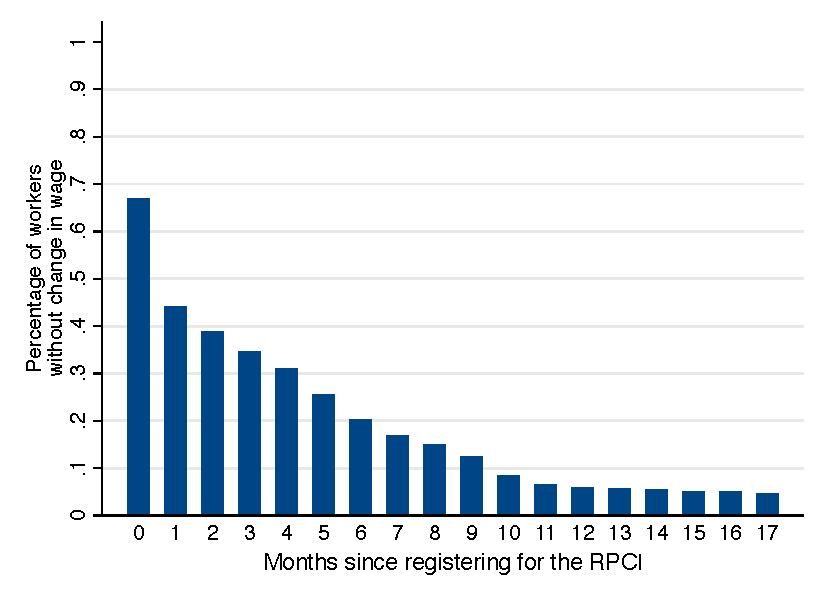
\includegraphics[width=\textwidth]{04_Figures/muestra_1porciento/hist_wage_time_since_treated_treat.pdf}
    \end{subfigure}
    \begin{subfigure}{0.49\textwidth}
    \caption{Control: after registering for the RPCI}
    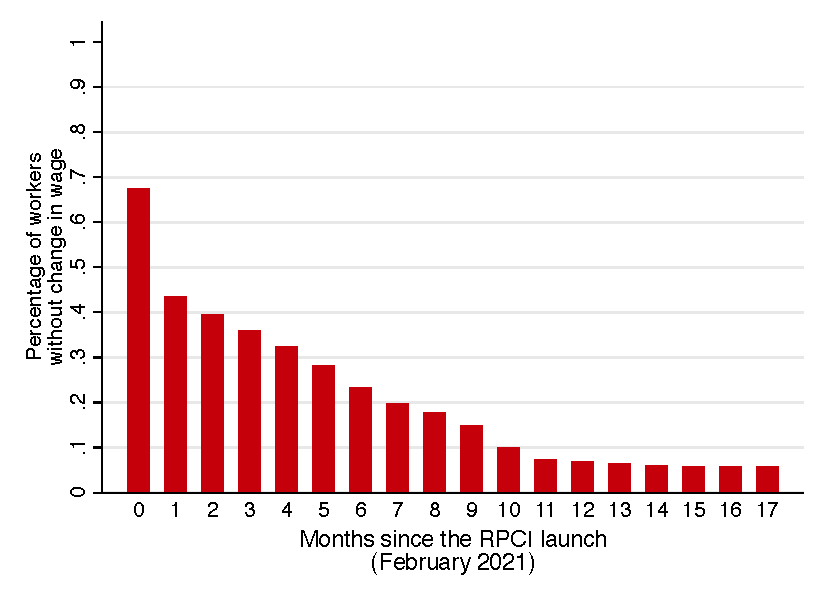
\includegraphics[width=\textwidth]{04_Figures/muestra_1porciento/hist_wage_time_since_treated_control_matched.pdf}
    \end{subfigure}
    
    \begin{subfigure}{0.49\textwidth}
    \caption{Difference (pp.) of the percentage of workers having the same wage by treatment status}
    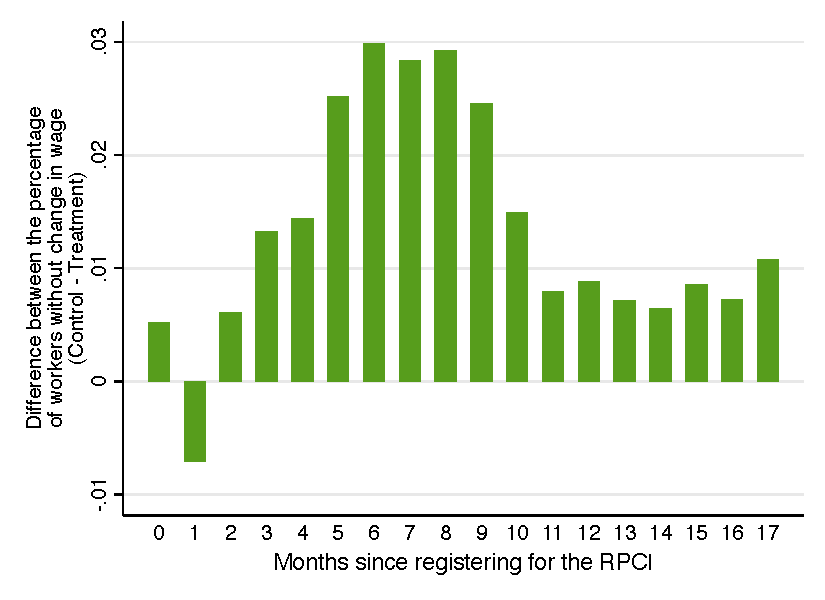
\includegraphics[width=\textwidth]{04_Figures/muestra_1porciento/hist_wage_time_since_treated_diff_matched.pdf}
    \end{subfigure}
    
    %\textit{Do file: hist_wage_time_since_treated.do}
    \end{center}
\end{figure}
\scriptsize{
\noindent This figure explores over time if workers that registered for the RPCI change their wages faster than workers who didn't register for the RPCI. The figures plot the percentage of workers that have the same wage after $t$ months. The workers that didn't register for the RPCI get the register date from the matched worker that did register for the RPCI, using nearest neighbor matching on the worker's baseline characteristics. \textit{Sample:} 1\% of the workers registered at the Mexican Institute of Social Security (IMSS) between January 2020 and August 2022. For the treatment group, compares the wage the worker had one month before registering for the RPCI with the wage after $t$ months of the register. For the control group, compares the wage the worker had one month before their matched treated worker registered for the RPCI, with the wage after $t$ months of the register. The y-axis measures the percentage of workers observed $t$ months with the same wage as in $t = -1$. Figure (c) present the difference between the bars in figures (b) and (a).
}


\clearpage

\begin{figure}[H]
    \caption{RPCI effect by cohort}
    \label{twfe_beta_cohort}
    \begin{center}
    
    \begin{subfigure}{0.49\textwidth}
    \caption{Effect on wage}
    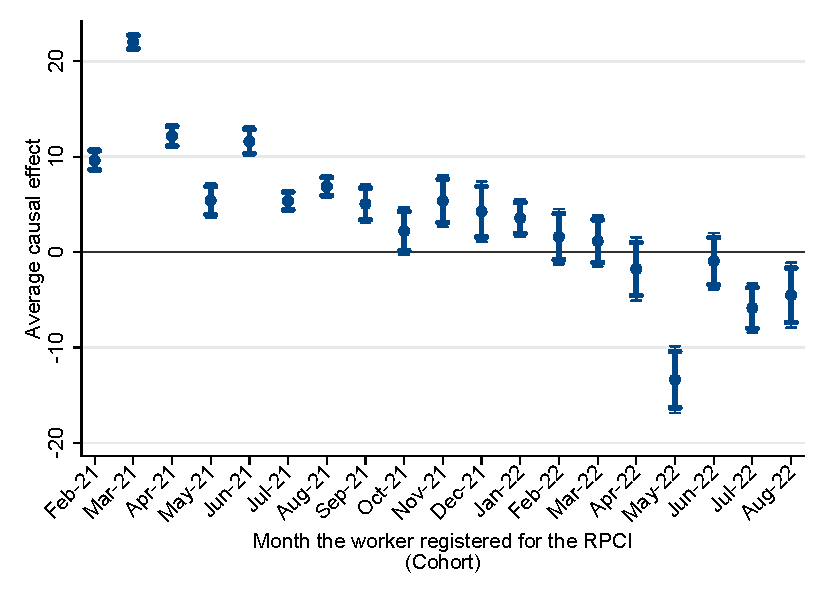
\includegraphics[width=\textwidth]{04_Figures/muestra_10porciento/twfe_beta_cohort_sal_cierre.pdf}
    \end{subfigure}
    \begin{subfigure}{0.49\textwidth}
    \caption{Effect on log wage}
    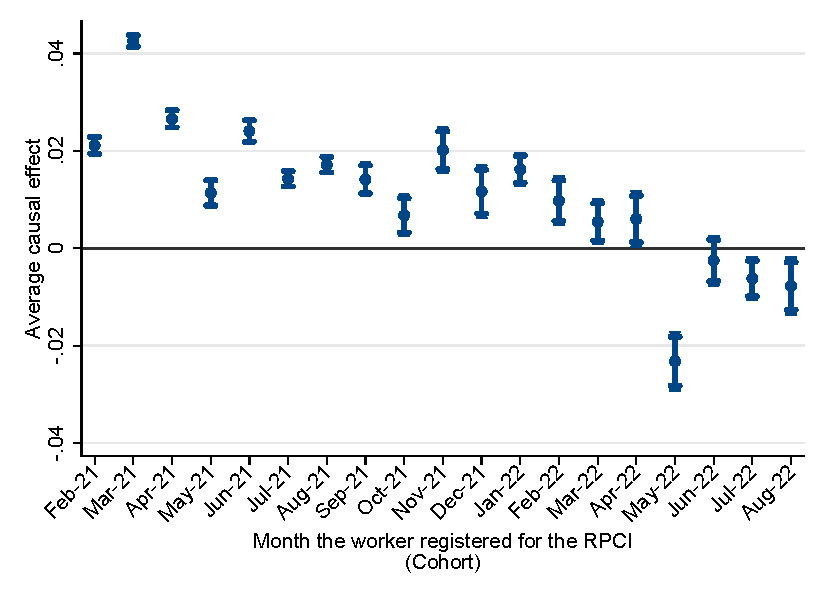
\includegraphics[width=\textwidth]{04_Figures/muestra_10porciento/twfe_beta_cohort_log_sal_cierre.pdf}
    \end{subfigure}
    
    %\textit{Do file: twfe_beta_cohort_rpci.do}
    \end{center}
\end{figure}
\scriptsize{
\noindent \textit{Sample:} 10\% of the workers registered at the Mexican Institute of Social Security (IMSS) between January 2020 and August 2022. Each point in the graph corresponds to the estimated regression coefficient where the sample conditions the treatment group by the cohort of register for the RPCI. All regressions have the same control group, meaning all samples include the workers who never registered for the RPCI. Regressions use the TWFE specification $y_{it} = \gamma_{i} + \theta_{t}+ \beta RPCI_{it} +\epsilon_{it}$, where $\gamma_{i}$ are dummies for each worker id, $\theta_{t}$ are dummies for each monthly period, and $RPCI_{it}$ are dummies where 1 means that the worker registered for the RPCI during that month or previous month, and include dummies for each state and dummies for each wage decile of the wage distribution during 2020, both interacted with dummies for each quarterly period. 
}

\clearpage

\begin{figure}[H]
    \caption{Event studies - RPCI effect on wage by cohort}
    \label{event_study_cohort}
    \begin{center}
    
    \begin{subfigure}{0.49\textwidth}
    \caption{Early adopters}
    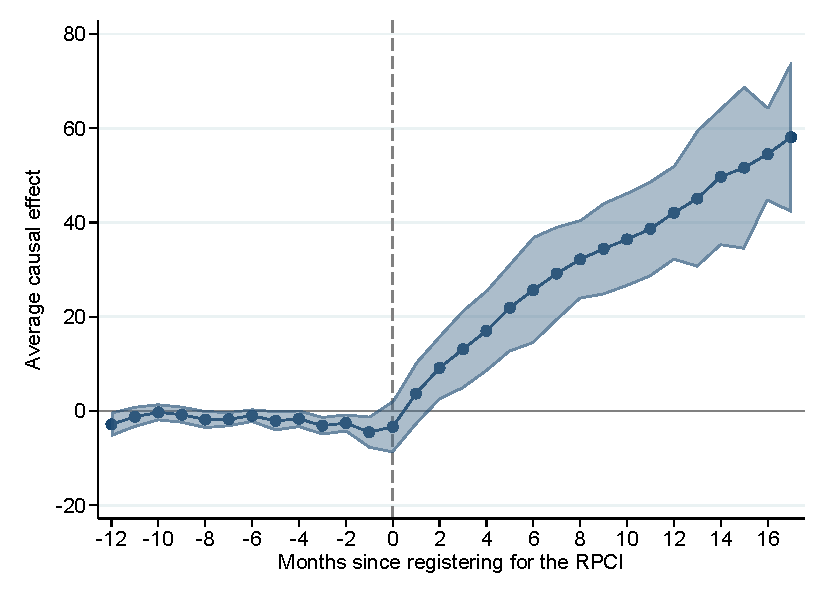
\includegraphics[width=\textwidth]{04_Figures/muestra_10porciento/event_study_sal_cierre_chaisemartin_adopters_early.pdf}
    \end{subfigure}
    \begin{subfigure}{0.49\textwidth}
    \caption{Late adopters}
    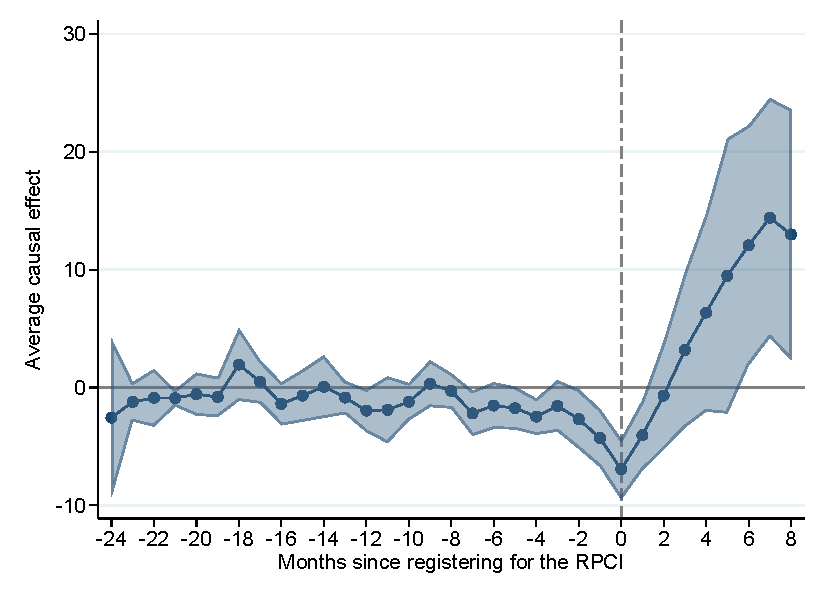
\includegraphics[width=\textwidth]{04_Figures/muestra_10porciento/event_study_sal_cierre_chaisemartin_adopters_late.pdf}
    \end{subfigure}
    
    
    %\textit{Do file: did_multiplegt_heterogeneity_rpci.do}
    \end{center}
\end{figure}
\scriptsize{
\noindent \textit{Sample:} 10\% of the workers registered at the Mexican Institute of Social Security (IMSS) between January 2020 and August 2022. The graphs use the estimators proposed by Chaisemartin and D'Haultfoeuille to prevent posible negative weights in the Difference in Differences estimators. Each subfigure conditions the treatment group by the cohort of register for the RPCI. Subfigure (a) conditions the treatment group to early adopters, meaning the workers who registered for the RPCI during the first nine months after the RPCI launch (February 2021 to October 2021). Subfigure (b) conditions the treatment group to late adopters, meaning the workers who registered for the RPCI during the next nine months (November 2021 to August 2022). Both subfigures have the same control group, meaning the workers who never registered for the RPCI. Subfigure (c) conditions the treatment group to early adopters and uses late adopters as control group.
}

\clearpage




%%%%%%%%%%%%%%%%%%%%%%%%%%%%%%%%%%%%%%%%%%%%%%%%%%%%%%

\newpage
%  \documentclass[oneside,11pt]{article}

% 
\usepackage{soul}
\usepackage{natbib}
\usepackage{hyperref}
\usepackage{bookmark}
\usepackage{graphicx}             
\graphicspath{{./Figuras/}}
\usepackage[dvipsnames]{xcolor}
\usepackage{todonotes}
\usepackage{makecell}
\usepackage[margin=1in]{geometry}
\usepackage{float}                
\usepackage{amsmath}
\usepackage{amscd}
\usepackage{amsfonts}
\usepackage{amssymb}
\usepackage{bbm}
\usepackage{booktabs}
\usepackage{nameref}
\usepackage{multirow}
\usepackage[nokeyprefix]{refstyle}
\usepackage{rotating}
\usepackage{threeparttable}
\usepackage{afterpage}
\usepackage{lscape}
\usepackage{enumerate}
\usepackage{caption}
\usepackage{subcaption}
\usepackage{epstopdf}
\usepackage{setspace}
\usepackage{svg}
\usepackage{dsfont}
\usepackage{amsthm}
\usepackage{tocloft}
\usepackage{etoc}
\usepackage{lmodern}
\usepackage{bm}
\usepackage[T1]{fontenc}
\usepackage{tgpagella}

\epstopdfDeclareGraphicsRule{.tiff}{png}{.png}{convert #1 \OutputFile}
\AppendGraphicsExtensions{.tiff}

\epstopdfDeclareGraphicsRule{.tif}{png}{.png}{convert #1 \OutputFile}
\AppendGraphicsExtensions{.tif}

\def\sym#1{\ifmmode^{#1}\else\(^{#1}\)\fi}

\usepackage{tikz}
\usetikzlibrary{shapes.geometric, arrows}
\usetikzlibrary{calc}
\usetikzlibrary{matrix}

\tikzset{ 
    table/.style={
        matrix of nodes,
        row sep=-\pgflinewidth,
        column sep=-\pgflinewidth,
        nodes={
            rectangle,
            draw=black,
            align=center
        },
        minimum height=1.5em,
        text depth=0.5ex,
        text height=2ex,
        nodes in empty cells,
%%
        every even row/.style={
            nodes={fill=gray!20}
        },
        column 1/.style={
            nodes={text width=2em,font=\bfseries}
        },
        row 1/.style={
            nodes={
                fill=black,
                text=white,
                font=\bfseries
            }
        }
    }
}


\usepackage{colortbl}
\usepackage{url}
\urlstyle{rm}
\definecolor{darkblue}{rgb}{0,0,.4}
\hypersetup{colorlinks=true, breaklinks=true, citecolor=Maroon, linkcolor=darkblue, menucolor=darkblue, urlcolor=darkblue}

\newtheorem{theorem}{Theorem}
\newtheorem{claim}[theorem]{Claim}
\newtheorem{prop}[theorem]{Proposition} 
\newtheorem{cor}[theorem]{Corollary} 
\newtheorem{assumption}{Assumption} 
\newtheorem{lem}{Lemma} 

\DeclareRobustCommand{\hlgr}[1]{{\sethlcolor{green}\hl{#1}}}


\usepackage{comment}
%para esconder columnas en tablas (enrique)
\usepackage{array}
\newcolumntype{H}{>{\setbox0=\hbox\bgroup}c<{\egroup}@{}}
\linespread{1.25}

\newcommand{\wh}{\widehat}
\usepackage{anyfontsize}

\usepackage[linesnumbered,vlined,ruled,commentsnumbered]{algorithm2e}

\DontPrintSemicolon
\newcommand{\To}{\mbox{\upshape\bfseries to}}
\newcommand{\E}{\mathbb{E}}

\DeclareCaptionFormat{cont}{#1 (cont.)#2#3\par}
% %%% HELPER CODE FOR DEALING WITH EXTERNAL REFERENCES
% \usepackage{xr}
% \makeatletter
% \newcommand*{\addFileDependency}[1]{
%   \typeout{(#1)}
%   \@addtofilelist{#1}
%   \IfFileExists{#1}{}{\typeout{No file #1.}}
% }
% \makeatother


% \newcommand*{\myexternaldocument}[1]{
%     \externaldocument{#1}
%     \addFileDependency{#1.tex}
%     \addFileDependency{#1.aux}
% }

% %\myexternaldocument{OA}

% %%%%%%%%%%%%%%%%%%%%%%%%%%%%%%%% DOCUMENT
% \begin{document}

%%%%%%%%%%%%%%%%%%%%%%%%%%%%%%%%%%%%%%%%%%%%%%%

% APPENDIX 
\setcounter{table}{0}
\setcounter{figure}{0}
\setcounter{section}{0}
\pagenumbering{gobble}


\begin{center}
	\LARGE IMSS RPCI \\[0.5em]
	\Large{Appendix $-$ For Online Publication} \\[1em]
	\large \author{Eduardo Alcaraz \and Gabriela López \and Luis Martínez \and Marco Medina \and Enrique Seira}
\end{center}

\appendix
\pagenumbering{arabic}
\renewcommand\thefigure{OA-\arabic{figure}}
\renewcommand\thetable{OA-\arabic{table}}
\renewcommand*{\thepage}{OA - \arabic{page}}
\renewcommand\thesection{Appendix \Alph{section}.}
\renewcommand\thesubsection{\Alph{section}.\arabic{subsection}}

%\renewcommand{\cftparskip}{0em} % NOT NEEDED
\renewcommand\cftsecdotsep{\cftdotsep}
\renewcommand\cftsubsecdotsep{\cftnodots}
\renewcommand{\cftsecnumwidth}{6em}
 \renewcommand{\cftpnumalign}{r}
%\renewcommand{\cftsecleader}{\normalfont\cftdotfill{\cftsecdotsep}}


\renewcommand{\cftsecleader}{\cftdotfill{\cftsecdotsep}\hspace{1.8em}}
%\renewcommand{\cftsecpagefont}{20em}
%\renewcommand{\cftfignumwidth}{6em}
%\renewcommand{\cfttabnumwidth}{3.3em}

%\tableofcontents
\etocdepthtag.toc{mtappendix}
\etocsettagdepth{mtchapter}{none}
\etocsettagdepth{mtappendix}{subsection}

\setstretch{0.9}
%\renewcommand\contentsname{} % the empty name

\begingroup
\let\clearpage\relax
%\vspace{-1.5em} % the removed space. Set as appropriate
\tableofcontents
\endgroup

\clearpage

\section{ RPCI}
\vspace{.2in}

\begin{figure}[H]
    \caption{RPCI flyers}
    \label{rpci_flyers}
    \begin{center}
    
    \begin{subfigure}{0.49\textwidth}
    \caption{RPCI flyer titled "Does my employer has me registered at IMSS?"}
    
\includegraphics[width=\textwidth]{04_Figures/rpci_app/rpci_flyer_3.jpeg}
    \end{subfigure}
    \begin{subfigure}{0.49\textwidth}
    \caption{RPCI flyer titled "Digital services for a healthy environment"}
    
\includegraphics[width=\textwidth]{04_Figures/rpci_app/rpci_flyer_2.jpeg}
    \end{subfigure}

    \end{center}
\end{figure}
\scriptsize{
\noindent Flyers circulated by the Mexican Institute of Social Security (IMSS) for the RPCI. Both flyers explain how you can track and access your job register information, such as wage and firm you are registered at, if you register for the RPCI.
}

\clearpage

\begin{figure}[H]
    \caption{Registering for the RPCI}
    \label{rpci_register}
    \begin{center}
    
    \begin{subfigure}{0.9\textwidth}
    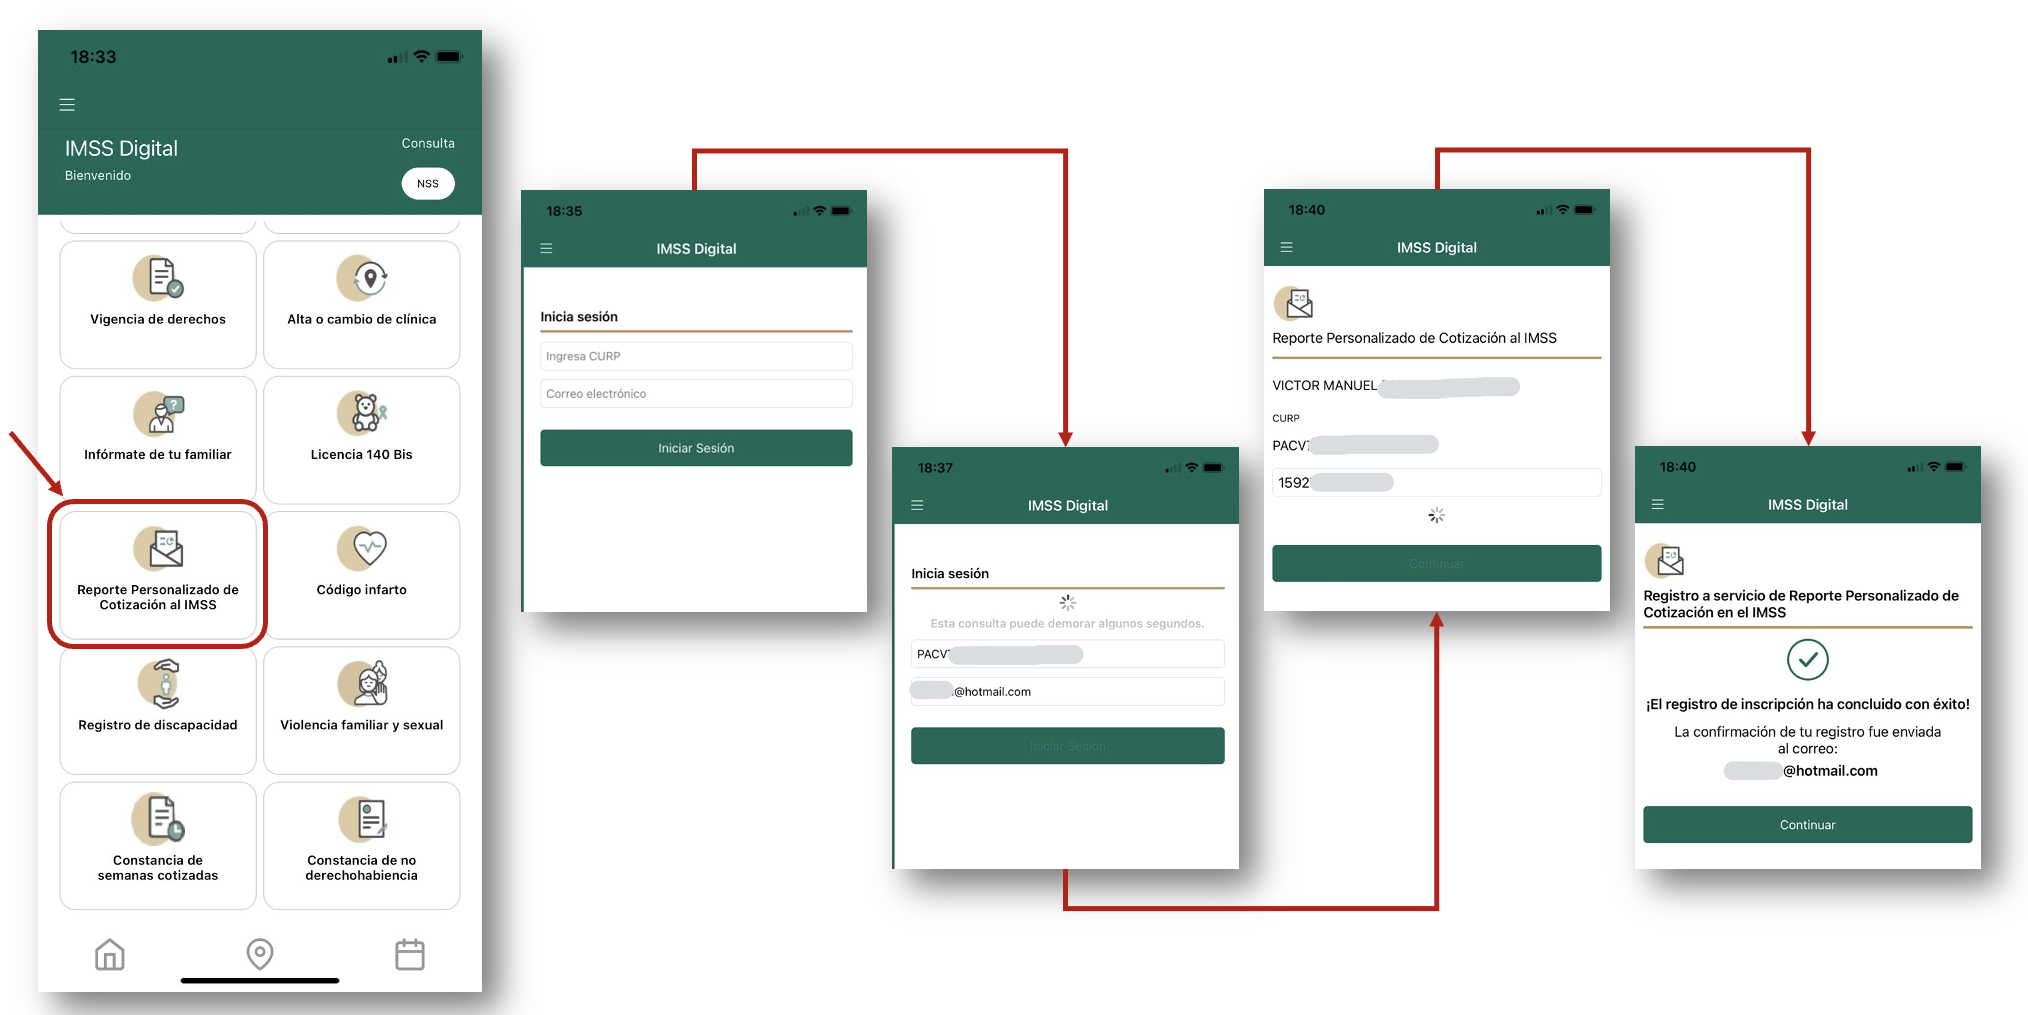
\includegraphics[width=\textwidth]{04_Figures/rpci_app/rpci_register.png}
    \end{subfigure}

    \end{center}
\end{figure}
\scriptsize{
\noindent Diagram shows how to register for the RPCI within the IMSS Digital app. The worker registers only once to access the RPCI, using his Unique Population Registry Key (CURP) and email address.
}

\clearpage

\begin{figure}[H]
    \caption{RPCI example}
    \label{rpci_example}
    \begin{center}
    
    \begin{subfigure}{0.49\textwidth}
    \caption{RPCI within the IMSS Digital app}
    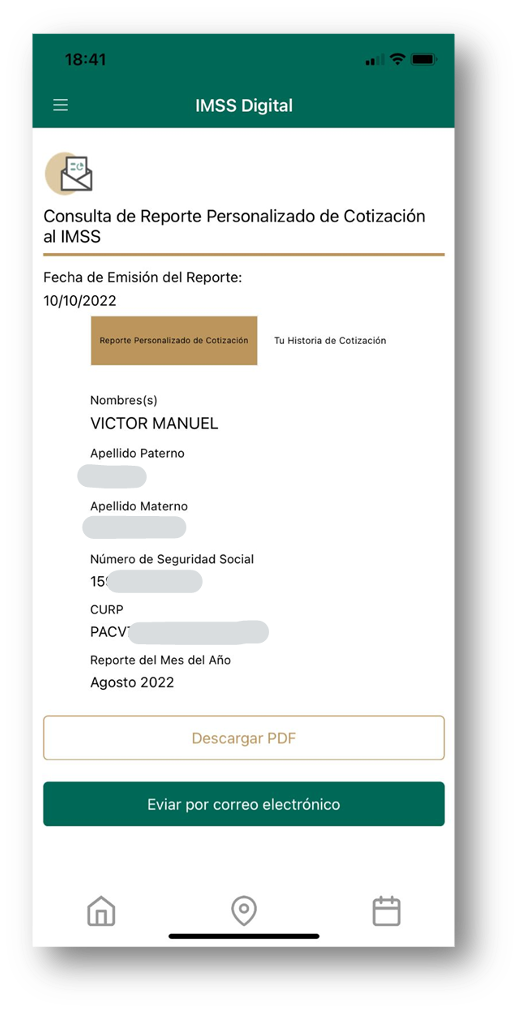
\includegraphics[width=\textwidth]{04_Figures/rpci_app/rpci_2.png}
    \end{subfigure}
    \begin{subfigure}{0.49\textwidth}
    \caption{RPCI PDF file}
    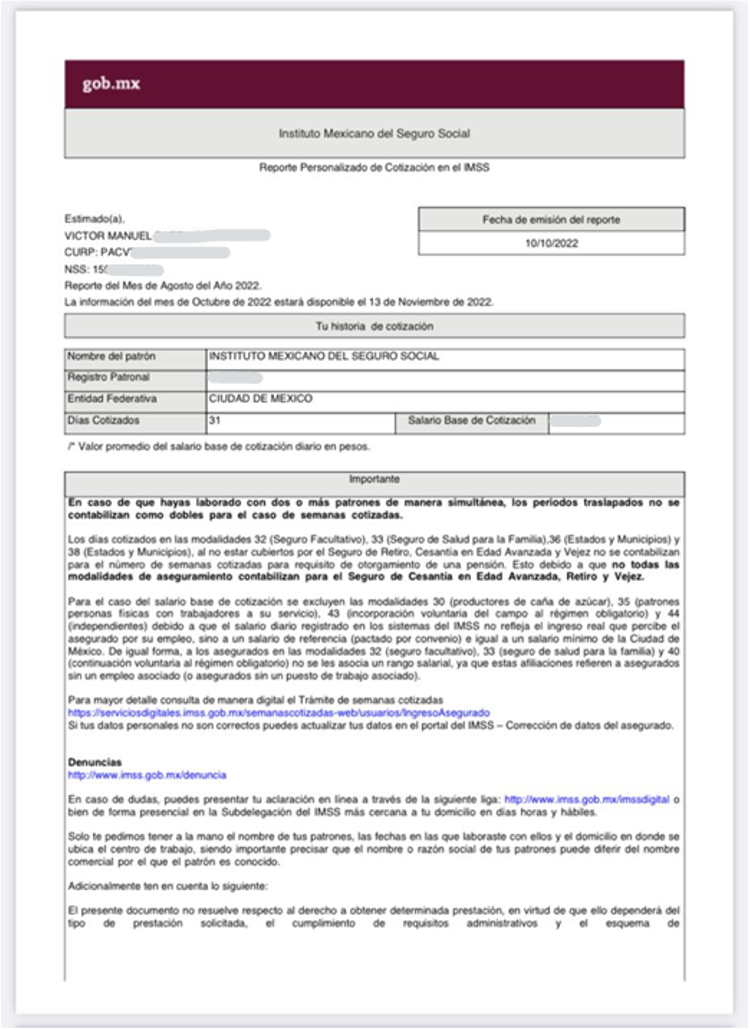
\includegraphics[width=\textwidth]{04_Figures/rpci_app/rpci_3.png}
    \end{subfigure}
    

    \end{center}
\end{figure}
\scriptsize{
\noindent Figure (a) shows the IMSS Digital app, where once the worker is registered for the RPCI, the worker can download their report in PDF or receive it via email. Figure (b) shows an example of the PDF for the RPCI. The report includes the worker job registered information, such as wage and the firm the worker is registered at.
}

%\clearpage

%\bibliographystyle{authordate1}
%\bibliographystyle{amsalpha}
%\bibliographystyle{AER}

%\bibliography{References}




% \end{document}

\end{document}

